\capitulo{5}{Aspectos relevantes del desarrollo del proyecto}

A la hora de realizar un proyecto de este tipo siempre surgen problemas o cuestiones que se han de ir resolviendo en ese momento, esta sección trata los puntos más relevantes.

\section{Concepto inicial del proyecto}
El proyecto planteado, en su forma inicial, trataba de la implementación de una aplicación de escritorio en lenguaje Python o Java permitiendo asignar semántica a las rutas analizadas.

Para ello, la aplicación debería poder leer y procesar ficheros de texto plano o csv. Todos los datos obtenidos serían almacenados en una Base de Datos PostgreSQL puesto que cuenta con una extensión llamada PostGIS que permite el análisis y tratamiento de posiciones geográficas añadiendo funcionalidad adicional al SGBD mencionado.

Puesto que la aplicación debía ser de fácil uso, se planteó una interfaz basada en Swing para poder mostrar los datos analizados así como mapas con las rutas procesadas.

Los primeros pasos orientados al diseño de la interfaz mediante Swing dejaron claro que no era la más adecuada ni sencilla para trabajar con mapas. Este es uno de los aspectos que animó a abandonar esta idea inicial por un desarrollo web cuya interfaz permite un manejo mucho más sencillo de todo tipo de mapas y librerías.

\section{Conocimientos previos}
A la hora de realizar este trabajo se contaban con algunos conocimientos previos  de programación web obtenidos a lo largo de los distintos cursos universitarios así como del desarrollo del Trabajo de Fin de Grado (basado en el CMS Drupal).

Aunque en esta ocasión el lenguaje elegido fue Java y se completó el desarrollo haciendo uso de páginas JSP y servlets. Por tanto, se tuvo que realizar un esfuerzo para aprender el manejo y programación mediante este lenguaje.

Adicionalmente, no se contaban con conocimientos sobre el funcionamiento de los sistemas de obtención de coordenadas ni de cómo podían ser tratados posteriormente.


\subsection{Coordenadas geográficas}
Debido a los distintos tipos de toma y representación de coordenadas geográficas es posible que una misma coordenada representada sobre distintos sistemas de mapas de lugar a errores de representación de varios centenares de metros. Este comportamiento puede observarse al comparar coordenadas geográficas presentadas por distintos motores de mapas. Por ejemplo, una coordenada localizada en China mostraba un mapa basado en Open Street Map no coincidirá con la misma coordenada mostrada por los mapas de Google.

Esto es así por el uso de distintos sistemas de coordenadas usados por ambos motores (EPSG:3857 en Google Maps frente a EPSG:4326 en OpenStreetMaps) \cite{epsg:wiki}.

Al comienzo del desarrollo del trabajo, no se conocían los diferentes sistemas de coordenadas dando lugar a confusión y errores en los cálculos sobre las rutas.

La Figura \ref{coordenadas} muestra la gran cantidad de sistemas de coordenadas disponibles a la hora de visualizar un fichero de puntos GPS o a la hora de obtener datos desde PostgreSQL.


\begin{figure}[h]
  \centering
    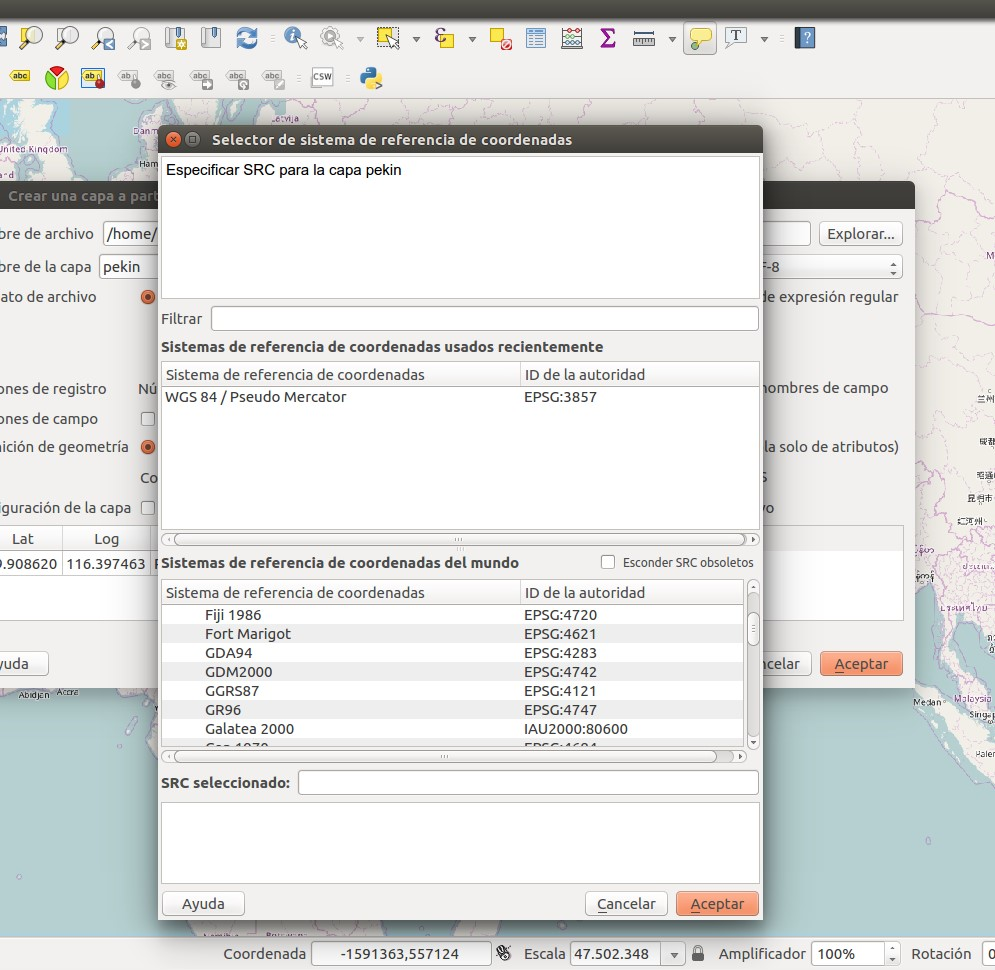
\includegraphics[width=0.6\textwidth]{../img/poi/qgis.jpg}
  \caption{Gran cantidad de sistemas de coordenadas en QGIS.}
  \label{coordenadas}
\end{figure}

\section{Errores propios del hardware}
Toda la tecnología GPS relacionada con el hardware cuenta con ciertas limitaciones, tanto en potencia de cálculo como en la toma de las posiciones en sí mismas.

Estas limitaciones favorecen la aparición de errores en las coordenadas medidas por cualquier hardware. Estos errores pueden hacer que la ruta tomada como verdadera contenga pequeños fallos en cada una de las coordenadas de las que está compuesta. Por este motivo, puede que una ruta inicialmente correcta indique un espacio recorrido mayor al realmente realizado o, incluso, marque puntos por los que no se han pasado.

Este echo puede ser fácilmente verificado atendiendo a las restricciones inherentes del hardware y a la forma en la que el software es implementado. Dejando un dispositivo GPS activo en un punto fijo, se verá al cabo de un cierto espacio de tiempo que el dispositivo parece moverse de forma autónoma. Este movimiento viene dado por los errores y/o fallos mencionados anteriormente.

Por tanto, es posible afirmar, que los datos con los que cada usuario cuenta tendrán un cierto error. Esto hace que los algoritmos de análisis y muestra de resultados deban tolerar estas inexactitudes. La Figura \ref{errores} muestra el movimiento virtual efectuado por dispositivo GPS completamente parado. \cite{pais:info}

\begin{figure}[h]
  \centering
    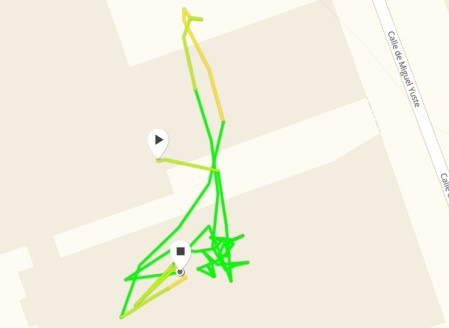
\includegraphics[width=0.6\textwidth]{../img/gps/errores.jpg}
  \caption{Movimiento }
  \label{errores}
\end{figure}

Estas restricciones han ocasionado que algunos conjuntos de datos no cuenten con la calidad suficiente para su uso en este trabajo así como que sus errores sean tan cuantiosos que las rutas no sean verosímiles.

\section{Obtención de datos}
Uno de las primeras cuestiones a resolver fue la búsqueda de datos que permitiesen dar comienzo al desarrollo del proyecto. Aunque existen gran variedad de \textit{datasets} en diversas páginas web dedicadas a su alojamiento, es cierto que no siempre cumplían con los requisitos necesarios para proceder a su análisis.

Algunos conjuntos de datos contaban con un buen número de ellos pero no contaban con ciertas características como una marca temporal para cada coordenada geográfica. Otros contaban con un buen número de características pero, en conjunto, resultaba un tamaño demasiado pequeño como para ser analizado.

Finalmente se encontró un conjunto de datos de Microsoft que, de forma general, satisfacía los requisitos que se habían marcado como mínimos siendo el usado para llevar a cabo las pruebas del sistema.

En este momento también comenzaron a surgir algunos de los problemas como los  que se indican en apartados inferiores.


\section{Tamaño de los datos de análisis}
Como ya ha sido comentado con anterioridad, el proyecto ha sido basado en una máquina virtual. Inicialmente se otorgó un tamaño estándar y fijo para el correcto desempeño de la distribución elegida. Pronto se tuvo constancia de que este tamaño no era suficiente. Aunque ya se habían instalado y configurado todos los componentes necesarios para el proyecto (PostgreSQL, PostGIS, NetBeans, etc.) no hubo otra opción que volver a crear una nueva máquina, esta vez con un tamaño mucho mayor y de espacio dinámico. Una vez reconfigurado todo el software necesario se pudo continuar con el normal desarrollo del trabajo.

No obstante y, como se describe a continuación, no solo crecía el tamaño en disco de todo el sistema, sino que también la Base de Datos aumentaba su volumen.

Antes de comenzar con las pruebas del sistema se cargó la Base de Datos con un completo conjunto de datos del mapa de China (los datos usados para las pruebas estaban basados en su gran mayoría en la ciudad de Pekín) viendo que el tamaño de las tablas era tan grande que ralentizaba cualquier intento de análisis de rutas.

En este momento se estaba llegando al límite de recursos de hardware que se podían asignar a la máquina virtual (llegando a contar con hasta 8 hilos, 10 GiB de RAM y un tamaño superior a las 100 GiB de espacio en disco). Se debía considerar otra aproximación que lograse una mejor experiencia y un mejor rendimiento.

Pronto se tuvo claro que no era necesaria tan elevada cantidad de datos y, que realmente, solo se usarían datos pertenecientes a la capa de Puntos De Interés. Es en este punto en el que se buscan herramientas para extraer estos PDIs de los ficheros de tipo osm descargados inicialmente. En esta búsqueda se encuentran las herramientas mencionadas en la sección anterior (Técnicas y herramientas).

De esta forma se logra disminuir el tamaño de unas tablas excesivamente grandes logrando una mejora del rendimiento global del sistema. Una vez iniciadas las pruebas del análisis de rutas del sistema se comprueba que el rendimiento ha experimentado una mejora real y se decide optar por mantener la estructura y conjunto de datos usados hasta el momento.


Como cabe esperar si finalmente la plataforma es puesta en producción, se hará uso de un servidor apropiado y con capacidades suficientes para que todo el sistema se comporte de forma correcta quedando disipado este problema .


\section{Tiempos de ejecución}
Ligado a los problemas mostrados en los apartados anteriores, los tiempos de ejecución eran tan elevados que, inicialmente, se necesitaban varias horas para obtener los primeros resultados. En estos momentos el hardware había llegado a su límite y no era posible una mayor asignación de recursos.

Una vez reducido el tamaño de los datos a consultar el rendimiento aumentó de forma considerable y ahora se pueden obtener los resultados esperados en pocos minutos.


\section{Diseño del algoritmo}
Durante los primeros pasos del proyecto se diseñó un algoritmo que incluía todos los pasos del mismo de forma secuencial. Es decir, todos los pasos debían ser ejecutados una vez se lanzase.

Este comportamiento no es el ideal puesto que el usuario puede tener la oportunidad de elegir los pasos que desea realizar sobre los datos que contienen sus ficheros. Por ejemplo, puede desear que sus datos no se mantengan en el sistema, que una ejecución busque PDIs pero otra solo paradas, etc.

Por tanto se decidió separar el algoritmo en diferentes clases que permitiesen una ejecución del algoritmo más personalizada.

Este hecho hizo que el desarrollo se viese ralentizado puesto que el cambio de la implementación del algoritmo implicó más tiempo del planeado inicialmente. Además, en este momento, se llevó a cabo la migración hacia la plataforma web, lo que implicó cambios adicionales sobre el código.

